Throughout the input specification the user is defining variables. As
described in the above sections many of these variables can be
specified by the user to be random variables. The UQ panel is where the user specifies the distribution of these random variables. Besides the properties of random variables, the sampling method and the number of requested samples shall also be defined by the user. The panel is split, as shown
in \Cref{fig:uq_panel}, into two frames:

\begin{enumerate}
\item Sampling Methods 
\item Random Variables
\end{enumerate}

\begin{figure}[!htbp]
  \centering {
    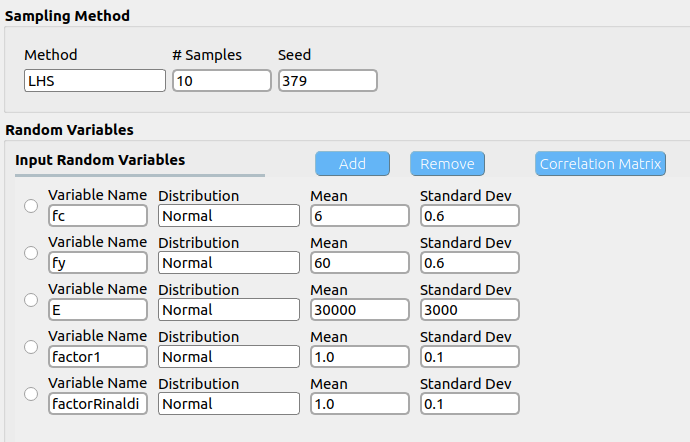
\includegraphics[width=0.8\textwidth]
    {usage/figures/uq1.png} }
  \caption{Uncertainty Quantification input panel}
  \label{fig:uq_panel}
\end{figure}

\subsection{Sampling Methods}
\input{usage/uq_forwardPropagationMethods}

\subsection{Random Variables}
The RV panel allows the user to specify the probabilistic distribution for the random problem at hand. The following probabilistic distributions for the random variables are currently supported: 
\begin{enumerate}
\item Gaussian
\item Lognormal
\item Beta
\item Uniform
\item Weibull
\item Gumbell
\end{enumerate}

Each distribution has different parameters, and the user needs to select accordingly the parameters for the distribution selected for each random variable. Once the user selects the distribution of the random variable, the
corresponding input boxes for the parameters will show. 

\Cref{fig:rv} shows the panel for a problem with four Random Variables with all random input following Gaussian distributions. 

\begin{figure}[!htbp]
  \centering {
    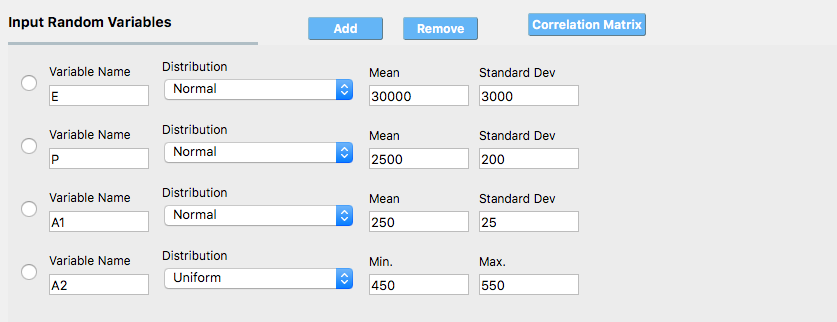
\includegraphics[width=0.8\textwidth]
    {examples/fig_quofem/rv.png} }
  \caption{Random Variable specification}
  \label{fig:rv}
\end{figure}



